\atsptt
    \begin{frame}{\ft{Using Dock Widgets For Flexible Layout}}
\section{Group 2: Using Dock Widgets For Flexible Layout}

        \begin{annotatedFigure}{0pt}{0pt}
            {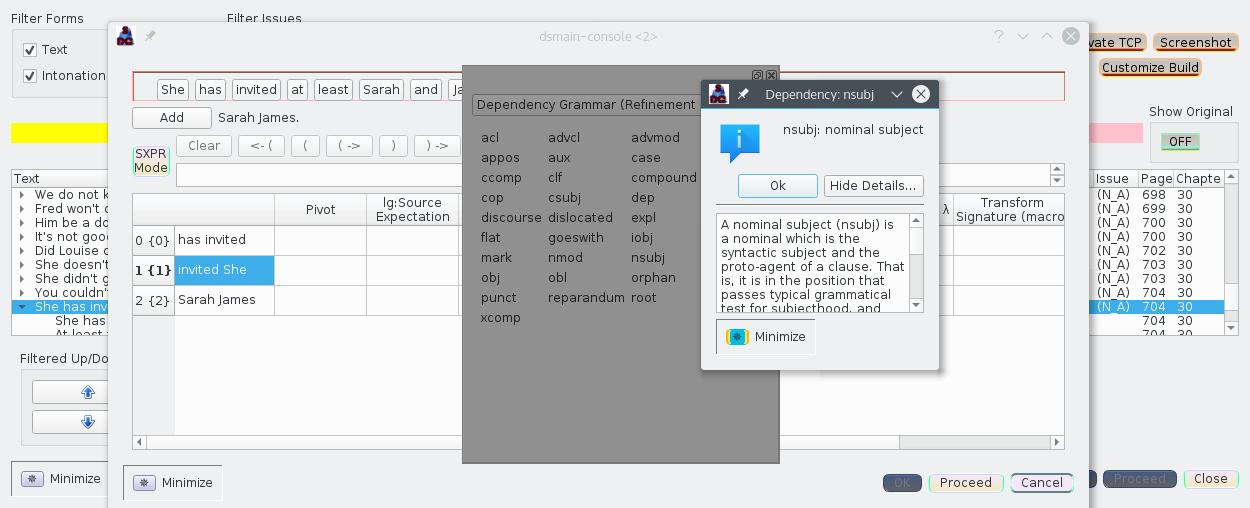
\includegraphics[scale=1]{texs/float.png}}
            
  \node [text width=7cm,inner sep=14pt,align=justify,
    draw = logoCyan!50!logoBlue,
    top color=logoCyan!40,text=black,
    bottom color=logoCyan!10,
    rounded corners=6pt,
  draw opacity=0.5,line width=1mm, fill opacity=0.9]
   at (0.25,0.73){\annfont\textbf{The 
   list of link/dependency relations is also isolated 
   as a ``dock widget" that may be dragged to float 
   above the other application windows  (\circled{1}), 
   or ``docked" at different positions (left or right) 
   on its parent window.  
   This screenshot also shows a dialog 
   box used for a precis of the individual 
   CoNLL-U (Conference on Natural 
   Language Learning - Universal) and Link
   Grammar relations (\circled{2}).}};


\annotatedFigureBox{0.37,0.23}{0.75,0.88}{1}{0.37,0.88}%                
\annotatedFigureBox{0.564,0.3}{0.75,0.84}{2}{0.564,0.84}%


\curicon{0.597}{0.32}

%\annotatedFigureBox{0.01,0.1}{0.55,0.334}{3}{0.55,0.334}            
            
      %      \annotatedFigureBox{0.222,0.284}{0.3743,0.4934}{B}{0.3743,0.4934}%tr
      %      \annotatedFigureBox{0.555,0.784}{0.6815,0.874}{C}{0.555,0.784}%bl
      %      \annotatedFigureBox{0.557,0.322}{0.8985,0.5269}{D}{0.8985,0.5269}%tr
  

  
        \end{annotatedFigure}

\end{frame}

